\section{A General Theory of Meaning}\label{sec:theory}

We present a general theory of meaning applicable across agent types (human, machine, etc.) and multimodal contexts. 
This theory does not aim to describe its own `implementation' in meaning-agents. 
Instead, this theory provides an efficacious model for discussing the many similarities between meaning-agents.
It is helpful to read this section as a genealogy of `social objects' such as values (fairness, liberty, equality) and social categories (race, class, gender).
%\jared{can cite hacking, looping effect}
% Citation moved as a concrete example to 'meaning in practice'
Such social objects begin, spurred on by context, inside the individual as abstract and become actualized over time.
%\andre{do you also want to mention the context? not just individual $\to$ world, but also world $\to$ individual}
Eventually, they enter into the shared social-material world, altering what was already there.
These social constructions begin to have material effects, which become new contexts that ground concretization.
``Social kinds'' are one prominent example of this ``looping effect'' \citep{Hacking:LoopingEffects}.
%, such as autism, disability, depression, and multiple-personality disorder.
% insofar as they regulate people, coming to change the way in which people mean.

% under a unified language.

%\markC{Possibly delete, not really necessary}
%As a methodological note, it is helpful to view many of the concepts in this paper as following binary structures that proceed from abstract to concrete. This general form is useful for framing many dichotomies in both the semiotic and ethical realms. A small list follows: Abstract $\to$ Concrete, Sign $\to$ Object, Concept $\to$ Context, Internal $\to$ External, Reification $\to$ Inscription, Concept $\to$ Content.

\begin{table}[!ht]
\centering
\begin{tabular}{l|l}
\toprule
Term            & Brief Description \\
\midrule
%Phenomenon      & A basic and independent unit of experience \\
Signification   & A relationship between two experiences, one of which picks out the other. \\
Context         & A material/social arrangement which imposes structure upon experience. \\
Sign            & An experience taken as signifying another experience. \\
Object          & An experience taken as being signified by another experience. \\
Concept         & An internalization of a context, regulating a set of sign-object relationships. \\
Determination   & The process of an object acquiring a signification. \\
Concretization  & A process of individual objects being determined by the context. \\
Inscription     & A process of altering the context through the exercise of concepts. \\
Social Totality  & The social arrangement governing a community of individuals. \\
\bottomrule
\end{tabular}
%\jared{Do we just mean people here or could the social totality refer also to a community of models e.g. in the recent alpaca farm paper?}
\end{table}

\subsection{Snapshots of meaning}\label{sec:theory:synchronics}

We will begin by discussing how our general theory of meaning operates at snapshots in time.
First, we start with pure individual experience in the snapshot before meanings emerge.
% We should immediately note something which will inevitably be found strange about the way we discuss experiences.
Importantly, according to our model of experience, all experiences begin by grasping a `thisness' of something \citep{Hegel:PhG}.
For example, suppose there is a table in a room.
The table might be brown, mottled with age, stained with food, etc.
This table has a variety of properties.
But an individual, upon first seeing the table, does not stop to pay attention to its brownness, its age, its uncleanliness, and so on.
Instead, this individual merely grasps that this table is a thing -- the `thisness' of the table.
If the individual has never seen a table before, they might not even grasp that it is in fact a table.
The individual's experience of the table is thus \textit{surprisingly empty}.
This experience has no internal contents or particularities, it just \textit{is}.
Because of this, we say that \textit{experiences begin as }\textbf{abstract}.
This initial abstractness of the experience allows us to avoid the pitfalls of qualia (ineffable, intrinsic, immediate, private \citep{Dennett:QuiningQualia} subjective experiences such as the redness of an apple).
%\jared{I like this example. Very solid.}

Over time, experiences become interrelated; they fall into certain roles with respect to one another.
Now, we will consider a snapshot wherein meanings have begun to develop -- that is, experiences have become related.
We call a relation between experiences a \textbf{signification}.
With a signification, one experience picks out another experience for an agent.
We call the experience that does the picking out the \textbf{sign}.
The experience being picked out is the \textbf{object} of that sign.
This description applies to all relations between experiences for any agent.
For an animal, a loud noise signifies a potential threat.
For humans using language, a name signifies a person.
The way in which the loud noise signifies the threat is very different from the way in which a name signifies a person.
The former does so through an automatic physiological response, the latter does so through language.
This `way of signifying' is the result of an external arrangement, social or material, imposing itself on experience.
For the animal, this arrangement is its evolutionary biology.
For a human using language, this arrangement is the language-game (a set of conventions that regulate the usage of language in a certain context \citep{Wittgenstein:PhilosophicalInvestigations}). 
This external arrangement is the \textbf{context}.
We might implicitly internalize the context (perhaps by learning the rules of the language-game over time).
A way of internalizing a context with respect to a set of meanings is a \textbf{concept}.
Over time, concepts enable individuals to develop more significations.
Thus, the central maxim of our theory is ``The \textbf{concept} makes possible the \textbf{signification} of the \textbf{object} by the \textbf{sign}.''
%This schema is simple but robust.
%Nevertheless, there are nuances we should explore.

%\andre{what if we just introduced each term after ``we posit a triad of sign concept object''} It behooves us to explore each term further:

\begin{figure}
    \centering
    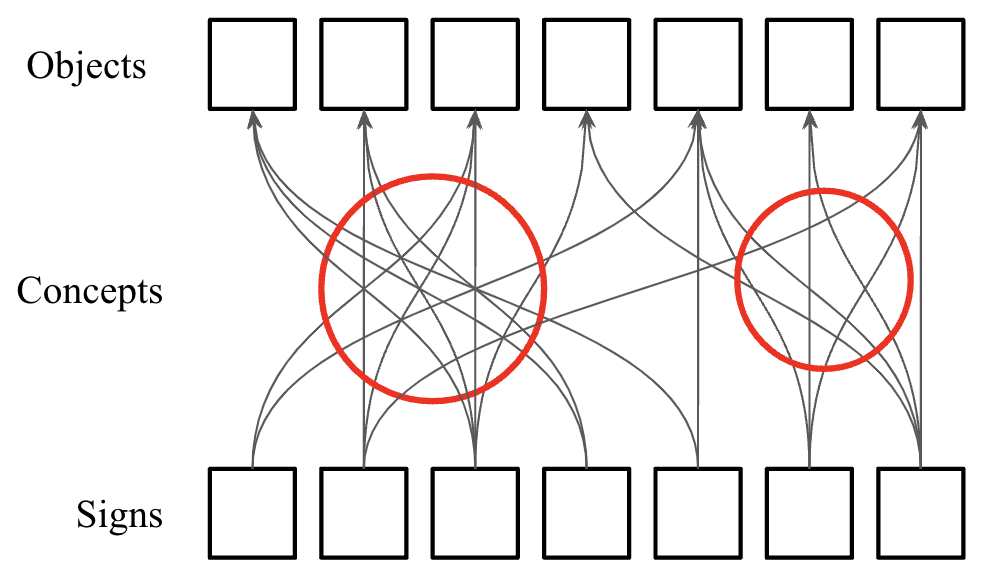
\includegraphics[width=6cm]{NeurIPS/imgs/sign-concept-object.png}
    \caption{Signification relations between \textit{signs} and \textit{objects}. Both signs and objects  have no internal content; they are determined by their relations ($\S$ \ref{sec:theory:synchronics}). Groups of significations are called \textit{concepts}.}
    \label{fig:enter-label}
\end{figure}

Recall that objects and signs are both just experiences. This allows us to explain meaning using only two sorts: \textit{experiences} and \textit{the relationships between experiences} (significations).\footnote{This two-sortedness bears a certain similarity to category theory with its notions of objects and morphisms. This is no accident \citep{Tsuchiya:CategoryTheoryNeuroscience}.
% Category theory determines objects wholly by their morphisms. It refuses to pry open the black box of what the object is. As will soon become clear, this external determination is the central paradigm of our theory of meaning.
}
This allows us to avoid complications with objects that do not exist in the material world.
Fictional characters are a classic example -- what does a name like ``Hamlet'' refer to? For our theory, it is the experiences signified by ``Hamlet.''
%\jared{I like this but possibly could cut from here to the end of the paragraph and keep the kripke citation}
% Perhaps the reader has constructed an impression of Hamlet in their mind.
% Perhaps the reader has seen a live performance of Hamlet and cannot get around `seeing' Hamlet as whoever played him. Each of these experiences is a potential object of the sign ``Hamlet.''
We also avoid the problem of whether proper names have descriptions or just tag their real objects by obviating the question of `real' referents entirely \citep{Kripke:NamingNecessity}.

\subsection{A genealogy of the object}\label{sec:theory:diachronics}
So far, our theory of meaning has provided the grounds for understanding how meaning operates at a single snapshot in time through four roles: the concept, the sign, the signification, and the object.
We now turn to the ways in which meaning applies itself over time to produce the object (i.e., its genealogy). 
Recall that we described experiences as initially abstract. 
Now, as experiences become objects of signs and signs for objects, they slowly become \textbf{concrete}. 
The original pure `thisness' is replaced by a rich concept, full of links to other experiences. 
Eventually, this concrete object enters the social-material world, thereby becoming fully concrete. 
These two processes are appropriately called \textbf{concretization} and \textbf{inscription}. 
Concretization is the process whereby an object becomes more concrete through acquiring significations. 
Each acquisition of a signification is called a \textbf{determination}.
More determined objects are thus more concrete.
%This allows us to speak of concrete objects as being more determined than abstract objects.
%\jared{as in no underdetermination at least for the meaning agent?}
Inscription is the process whereby individual meanings enter the social-material world. 
This is a process of realizing the object, actualizing what before only ever existed as an experience.

%\jared{there's something afoot in this section wrt who "we" are. I think you mean at times "we" as a society with pretheoretic notions of concept. but at other times in the paper you mean "we" as the authors of this paper.}
\paragraph{Concretization}
Our original usage of the term `concept' to mean an internalized context may seem strange. The term `concept' usually indicates an idea, something individuals have direct access to. Usually, this idea is thought of as having (or being) content. However, these two notions prove to be the same. First, we will understand how the colloquial notion appears in our theory. We do not discuss the \textit{internal} content of experiences, so experiences must instead acquire content by determination. This \textit{external} content is their concept. This comports with the colloquial sense of `concept': the concept of an experience is the things it signifies and the things that signify it. The concept of fairness is all things fairness means and all things that mean fairness. Fairness is what it is because it is (in part) impartiality and (in part) a standard by which to measure behavior (among other significations). The concept of fairness is described by an enumeration of its significations.

This definition of the concept (all the significations of an experience) aligns with our first definition of the concept (a way of internalizing a context).
Because a context is an external arrangement, it has a structure of `real' social or material objects and the relations between them \citep{Millikan:BeyondConcepts}. When these objects are experienced by individuals, they attempt to replicate this structure. The result of this replication is in fact the set of significations of experiences (our previous definition of concept).

Because concretization is a process of determination (acquiring significations), both the creation and adjustment of concepts are processes of concretization. Operationally, creation and adjustment differ heavily. Efficacious creation of a concept requires that the meaning-agent clearly prioritize a context. Once this prioritization is done, the actual creation follows as something simple. For example, the context ``the English language-game'' is prioritized
\footnote{There is a strong link between prioritization and intentionality via the notion of unitarity (see $\S$\ref{appendix:possibility}). 
}
% We anticipate the rejoinder that this prioritization is where we have hidden intentionality; this may well be true. We highlight this as an area for further development. However, we should note that by sequestering intentionality within prioritization, we have made a link between intentionality and unitarity  while allowing non-intentional systems of meaning to mean in non-unitary ways.
% \jared{Try to shorten this to two lines.}
; a word such as `table' is determined against an object, a `real' table (potentially) in the world, therefore becoming concretized.
However, a failure to adequately prioritize a context can result in scattered, non-efficacious concepts.
Adjustment, however, occurs under a predetermined context. If `table' is made to refer to all tables instead of just a singular table in the world, the original determination continues to exist under a different context.

\paragraph{Inscription}
Broadly speaking, inscription is the process of writing objects into the world -- creating or altering social material objects that correspond to experiential objects. \textit{However, inscription is not as simple as a direct transfer from the experiential world to the social-material world}. This may seem problematic -- after all, communication depends entirely on inscription. However, since communication is possible, we can infer that inscription must have certain properties.

% \jared{I might cut this paragraph and then put the quine citation on the first sentence of the next paragraph}
% One common paradigm in linguistics and semiotics is that meaning consists in reference to real (social or material) objects. If two subjects communicating are not referring to the same real object by the same term, they do not mean the same thing. As an example, this assumption grounds the theoretical impossibility of translation \citep{Quine:WordObject}. Two subjects using different languages have different sets of referents. We claim that even subjects using the same language have different sets of referents.

For meaning to be possible, we posit that meaning can in fact function when the referents of terms in a language are underdetermined. In fact, \textit{meaning is always underdetermined} \cite{Quine:WordObject}. Because objects are externally determined, communicators are always referring to any number of potential social or material objects. Meaning happens when relations between these social or material objects correspond to relations between experiential correlates (of these social or material objects) for both communicators. This correspondence is precisely what inscription must then produce. We claim, then, that \textit{in a vacuum (with no other social or material forces), inscription by a meaning-agent produces social or material objects with determinations that correspond to the determinations of experience for that meaning-agent}. This is our ``postulate of inscription.''

%\jared{these are no longer external, "social or material" objects but are rather internal experiential objects, right? Need some clarification here or above}
%\jared{Maybe part of my problem is not being clear on what you mean by 'social-material'}
The material objects created by inscription are totally concrete (in contrast to their experiential correlates). All possible properties (e.g. location, time, composition) are determined. Some of these determinations happen arbitrarily because they have no correlate in the mind. For example, the chemical makeup of the paint in a painting is usually not determined for the painter.

This gives us \textit{a genealogy of the object}: the object begins in the experiential world as totally abstract, an undetermined `thisness'. Over time, it accrues determinations, becoming gradually more concrete. Eventually, it proceeds out into the social-material world, where it is at its most concrete. This procession redetermines the structures of the social-material world, creating a cyclic effect whereby inscription by agents conditions future concretization.

\subsection{The social object}\label{sec:theory:social}
This theory of meaning also gives us the appropriate tools to describe the object as it passes beyond the experiential world and into the social (material) world -- in other words, the object as a \textbf{social object}. This discussion of the social object will prefigure our forthcoming analysis of values and categories insofar as they are themselves social objects -- most pertinently, for example, morality.
%, but also gender, race, class, etc.

Recall our ``postulate of inscription'': inscription reproduces the determinations of the object it inscribes.
%Under this assumption, material objects can continue to have internal contents which may or may not be perceptible, but remain structurally perceptible via their external determinations.\footnote{This idea of a material structure of objects is broadly similar to the ontology of right-wing Sellarsians (i.e. Milikan).}
Now, consider a material object. It has a variety of determinations -- color, location, composition, and so on. Only some of these are ever experienced by individuals. The sum of these experiences determines a \textit{social} object. In general, a social object is a sum of determinations over individuals in a society. It is reasonable to ask in what sense the social object `really' exists. Who is the social object an object for? We claim that it is useful to posit an abstract model of society as a meaning-agent. We can treat this abstraction much like we treat individuals. It has its own concepts, signs, and objects. We do not have to be ontologically committed to its existence for it to be useful. Generally speaking, this abstraction is something like our collective ground of meaning as a society.

We give this abstraction the name \textbf{social totality}, emphasizing its nature as a system of meaning. Then, \textit{the objects of the social totality are the social objects.} \textit{Moreover, the }\textbf{concepts}\textit{ of the social totality are many of the }\textbf{contexts}\textit{ about which we have been writing.} For example, the language-game, which operates as as \textit{context} for an individual, is a \textit{concept} for the social totality \citep{Gadamer:TruthAndMethod, Heidegger:BeingAndTime}. \textit{In fact, all social contexts are concepts of the social totality.} This means that the social totality accrues a variety of concepts in which to determine objects.

% This social totality is an abstraction -- we do not need to be ontologically committed to its existence -- but it is useful insofar as it allows us to analogize between our own common ground of meaning and ourselves as experiencing beings. 
% Although we do not need to be ontologically committed to it, the concept of social totality and our own ground of experience have the same structure of meaning.
%Both our individual and collective grounds of meaning (the latter being the ``social totality'') have the same structure: that of sign, concept, and object.
%Under this structure, the social totality has as its \textit{objects} precisely these social objects in abstract.
%Its \textit{determinations} are the determinations which we inscribe into its corpus (in a literal and textual sense). 
%Its objects are \textit{determined} by those individual significations which we inscribe into the corpus of the social totality. 
%\jared{How is this inscription occurring?}
%Its internal concepts are in fact what we have called contexts; contexts are the concepts of the social totality.

Because of this diversity of concepts, when considered as a meaning-agent, the meanings of the social totality are highly indeterminate. Thus, the social totality is perpetually in conflict with itself. This constant struggle is the social history of the object~\citep{foucault2002order}. In a certain sense, then, the truth of social totality is eternal self-contradiction~\citep{Hegel:PhG}. But it is a powerful kind of self-contradiction comprised by multitudes of information grouped according to their contexts. So we must be precise: to understand the contradiction involved in a concept, we must understand the histories, peoples, and diverse points of view which go into making a concept what it is. 

Let us now consider an example: how does a child learn what `fairness' means? `Fairness' begins as a social structure -- a \textit{social object} for the \textit{social totality}. A child learns certain things from their society about norms of behavior.
%They begin to relate instinctual \textit{experiences} of being wronged to fairness.
Slowly, they develop a \textit{concept} of effort as ``fairly'' \textit{signifying}' reward \citep{Rawls:TheoryJustice}. These concepts -- norms, deservingness, etc. -- amalgamate around the word `fairness' as `fairness' is \textit{concretized}. When this child says, ``That's unfair!'', they are doing more than pointing out some behavior that violates the norms. They also invoke all concepts with which `fairness' is related. Finally, the way this child writes and acts will reflect the myriad ways they perceive ``fairness'' as an aggregate of many experiences. The potential misconceptions or priorities this child has about fairness will go back into the world -- they will be \textit{inscribed}.

%\subsection{Meaning in practice}

%This $\S$ will be a gloss of the meaning-theory in practice which covers a single instance of `what meaning is' accounting for communication, reification, etc.

%\andre{Would be nice to have a small sentence at the bottom here just saying something like ``meaning is ...'' -- maybe like ``the interplay between sign, object, and concept. For example, the meaning of ``pass the salt please'' is the interplay between how it appears in my phenomenal experience, the conceptual intermdiary it signs trhough, and the object of the signing (an action impelled).''}
